% THIS IS AN EXAMPLE DOCUMENT FOR VLDB 2012
% based on ACM SIGPROC-SP.TEX VERSION 2.7
% Modified by  Gerald Weber <gerald@cs.auckland.ac.nz>
% Removed the requirement to include *bbl file in here. (AhmetSacan, Sep2012)
% Fixed the equation on page 3 to prevent line overflow. (AhmetSacan, Sep2012)

\documentclass{vldb}
\usepackage{graphicx}
\usepackage{balance}  % for  \balance command ON LAST PAGE  (only there!)
\usepackage{fontspec}
\usepackage{hyperref}
\graphicspath{{figures/}}
\usepackage{enumitem}

\begin{document}

% ****************** TITLE ****************************************

\title{The RADStack: Open Source Lambda Architecture for Interactive Analytics}

% possible, but not really needed or used for PVLDB:
%\subtitle{[Extended Abstract]
%\titlenote{A full version of this paper is available as\textit{Author's Guide to Preparing ACM SIG Proceedings Using \LaTeX$2_\epsilon$\ and BibTeX} at \texttt{www.acm.org/eaddress.htm}}}

% ****************** AUTHORS **************************************

% You need the command \numberofauthors to handle the 'placement
% and alignment' of the authors beneath the title.
%
% For aesthetic reasons, we recommend 'three authors at a time'
% i.e. three 'name/affiliation blocks' be placed beneath the title.
%
% NOTE: You are NOT restricted in how many 'rows' of
% "name/affiliations" may appear. We just ask that you restrict
% the number of 'columns' to three.
%
% Because of the available 'opening page real-estate'
% we ask you to refrain from putting more than six authors
% (two rows with three columns) beneath the article title.
% More than six makes the first-page appear very cluttered indeed.
%
% Use the \alignauthor commands to handle the names
% and affiliations for an 'aesthetic maximum' of six authors.
% Add names, affiliations, addresses for
% the seventh etc. author(s) as the argument for the
% \additionalauthors command.
% These 'additional authors' will be output/set for you
% without further effort on your part as the last section in
% the body of your article BEFORE References or any Appendices.

\maketitle

\begin{abstract}
\textit{The Real-time Analytics Data Stack, colloquially referred to
as the RADStack, is an open-source data analytics stack designed to provide
fast, flexible queries over up-to-the-second data. It is designed to overcome
the limitations of either a purely batch processing system (it takes too
long to surface new events) or a purely real-time system (it's difficult to
ensure that no data is left behind and there is often no way to correct data
after initial processing). It will seamlessly return best-effort results on
very recent data combined with guaranteed-correct results on older data. In
this paper, we introduce the architecture of the RADStack and discuss our
methods of providing interactive analytics and a flexible data processing
environment to handle a variety of real-world workloads.}
\end{abstract}

\section{Introduction}
The rapid growth of the Hadoop\cite{shvachko2010hadoop} ecosystem has enabled
many organizations to flexibly process and gain insights from large quantities
of data. These insights are typically generated from business intelligence, or
OnLine Analytical Processing (OLAP) queries. Hadoop has proven to be an
extremely effective framework capable of providing many analytical insights and
is able to solve a wide range of distributed computing problems. However, as
much as Hadoop is lauded for its wide range of use cases, it is derided for its
high latency in processing and returning results. A common approach to surface
data insights is to run MapReduce jobs that may take several hours to complete.

Data analysis and data-driven applications are becoming increasingly important
in industry, and the long query times encountered with using batch frameworks
such as Hadoop are becoming increasingly intolerable. User facing applications
are replacing traditional reporting interfaces as the preferred means for
organizations to derive value from their datasets. In order to provide an
interactive user experience with data applications, queries must complete in an
order of milliseconds. Because most of these interactions revolve around data
exploration and computation, organizations quickly realized that in order to 
support low latency queries, dedicated serving layers were necessary. Today,
most of these serving layers are Relational Database Management Systems (RDBMS)
or NoSQL key/value stores. Neither RDBMS nor NoSQL key/value stores are
particularly designed for analytics \cite{stonebraker2009requirements}, but
these technologies are still frequently selected as serving layers. Solutions
that involve these broad-focus technologies can be inflexible once tailored to
the analytics use case, or suffer from architecture drawbacks that prevent them
from returning queries fast enough to power interactive, user-facing
applications \cite{tschetter2011druid}.

An ideal data serving layer alone is often not sufficient as a complete analytics
solution. In most real-world use cases, raw data cannot be directly stored in
the serving layer. Raw data suffers from many imperfections and must first be
processed (transformed, or cleaned) before it is usable
\cite{stonebraker2010mapreduce}. The drawback of this requirement is that
loading and processing batch data is slow, and insights on events cannot be
obtained until hours after the events have occurred.

To address the delays in data freshness caused by batch processing
frameworks, numerous open-source stream processing frameworks such as Apache
Storm\cite{marz2013storm}, Apache Spark Streaming\cite{zaharia2012discretized},
and Apache Samza\cite{2014samza} have gained popularity for offering a
low-latency model to ingest and process event streams at near real-time speeds.
The drawback of almost all stream processors is that they do not
necessarily provide the same correctness guarantees as batch processing
frameworks. Events can come in days late, and may need to be corrected after
the fact. Large batches of data may also need to be reprocessed when new
columns are added or removed.

Combining batch processing, streaming processing, and a serving layer in a
single technology stack is known as a lambda
architecture\cite{hausenblas2014lambda}. In lambda architectures, data entering
the system is concurrently fed to both the batch and streaming processing
layer. The streaming layer is responsible for immediately processing incoming
data, however, the processed data may suffer from duplicated events and other
imperfections in data accuracy. The batch layer processes incoming data much
slower than the streaming layer, but is able to provide accurate views of data.
The serving layer merges the results from the batch and streaming layers and
provides an interface for queries. Although each individual component in a
lambda architecture has their own limitations, the pieces complement each other
extremely well and the overall stack is robust enough to handle a wide array of
data processing and querying challenges at scale. 

The RADStack is an open source lambda architecture implementation meant to offer flexible,
low-latency analytic queries on near real-time data. The solution combines the
low latency guarantees of stream processors and the correctness and flexibility
guarantees of batch processors. It also introduces a serving layer specifically
designed for interactive analytics. The stack’s main building blocks are Apache
Kafka\cite{kreps2011kafka}, Apache Samza, Apache Hadoop, and Druid
\cite{yang2014druid}, and we have found that the combination of technologies is
flexible enough to handle a wide variety of processing requirements and query
loads. Each piece of the stack is designed to do a specific set of things very
well. This paper will cover the details and design principles of the RADStack.
Our contributions are around the architecture of the stack itself, the
introduction of Druid as a serving layer, and our model for unifying real-time
and historical workflows.

The structure of the paper is as follows: Section \ref{sec:background}
describes the problems and use cases that led to the creation of the RADStack.
Section \ref{sec:serving} describes Druid, the serving layer of the stack, and
how Druid is built for real-time and batch data ingestion, as well as
exploratory analytics. Section \ref{sec:processing} covers the role of Samza
and Hadoop for data processing, and Section \ref{sec:delivery} describes the
role of Kafka for event delivery. In Section \ref{sec:performance}, we present
our production metrics.  Section \ref{sec:experiences} presents our experiences
with running the RADStack in production, and in Section \ref{sec:related} we
discuss the related solutions.

\section{Background}
\label{sec:background}

\begin{table*}
\centering
\begin{tabular}{| l | l | l | l | l | l | l | l |}
  \hline
  \textbf{Timestamp} & \textbf{Publisher} & \textbf{Advertiser} & \textbf{Gender} & \textbf{City} & \textbf{Click} & \textbf{Price} \\ \hline
  2011-01-01T01:01:35Z & bieberfever.com & google.com & Male & San Francisco & 0 & 0.65 \\ \hline
  2011-01-01T01:03:63Z & bieberfever.com & google.com & Male & Waterloo & 0 & 0.62 \\ \hline
  2011-01-01T01:04:51Z & bieberfever.com & google.com & Male & Calgary & 1 & 0.45 \\ \hline
  2011-01-01T01:00:00Z & ultratrimfast.com & google.com & Female & Taiyuan & 0 & 0.87 \\ \hline
  2011-01-01T02:00:00Z & ultratrimfast.com & google.com & Female & New York & 0 & 0.99 \\ \hline
  2011-01-01T02:00:00Z & ultratrimfast.com & google.com & Female & Vancouver & 1 & 1.53 \\ \hline
\end{tabular}
\caption{Sample ad data. These events are created when users views or clicks on ads.}
\label{tab:sample_data}
\end{table*}

The RADStack was first developed to address problems in the online advertising.
In online advertising, automated systems from different organizations will
place bids against one another to display users ads in the milliseconds before
a webpage loads. These actions generate a tremendous volume of data. The data
shown in Table~\ref{tab:sample_data} is an example of such data.  Each event is
comprised of three components: a timestamp indicating when the event occurred;
a set of dimensions indicating various attributes about the event; and a set of
metrics concerning the event. Organizations frequently serve this insights to
this data to ad publishers through visualizations and data applications. These
applications must rapidly compute drill-down and aggregates with this data, and 
answer questions such as “How many clicks occurred over the span of one week
for publisher google.com?” or “How many impressions were seen over the last
quarter in San Francisco?”. Queries over any arbitrary number of dimensions
should return in a few hundred milliseconds.

As an additional requirement, user-facing applications often face highly
concurrent workloads and good applications need to provide relatively
consistent performance to all users.  Of course, backend infrastructure also
needs to be highly available. Downtime is costly and many businesses cannot
afford to wait if a system is unavailable in the face of software upgrades or
network failure.

\begin{figure}
\centering
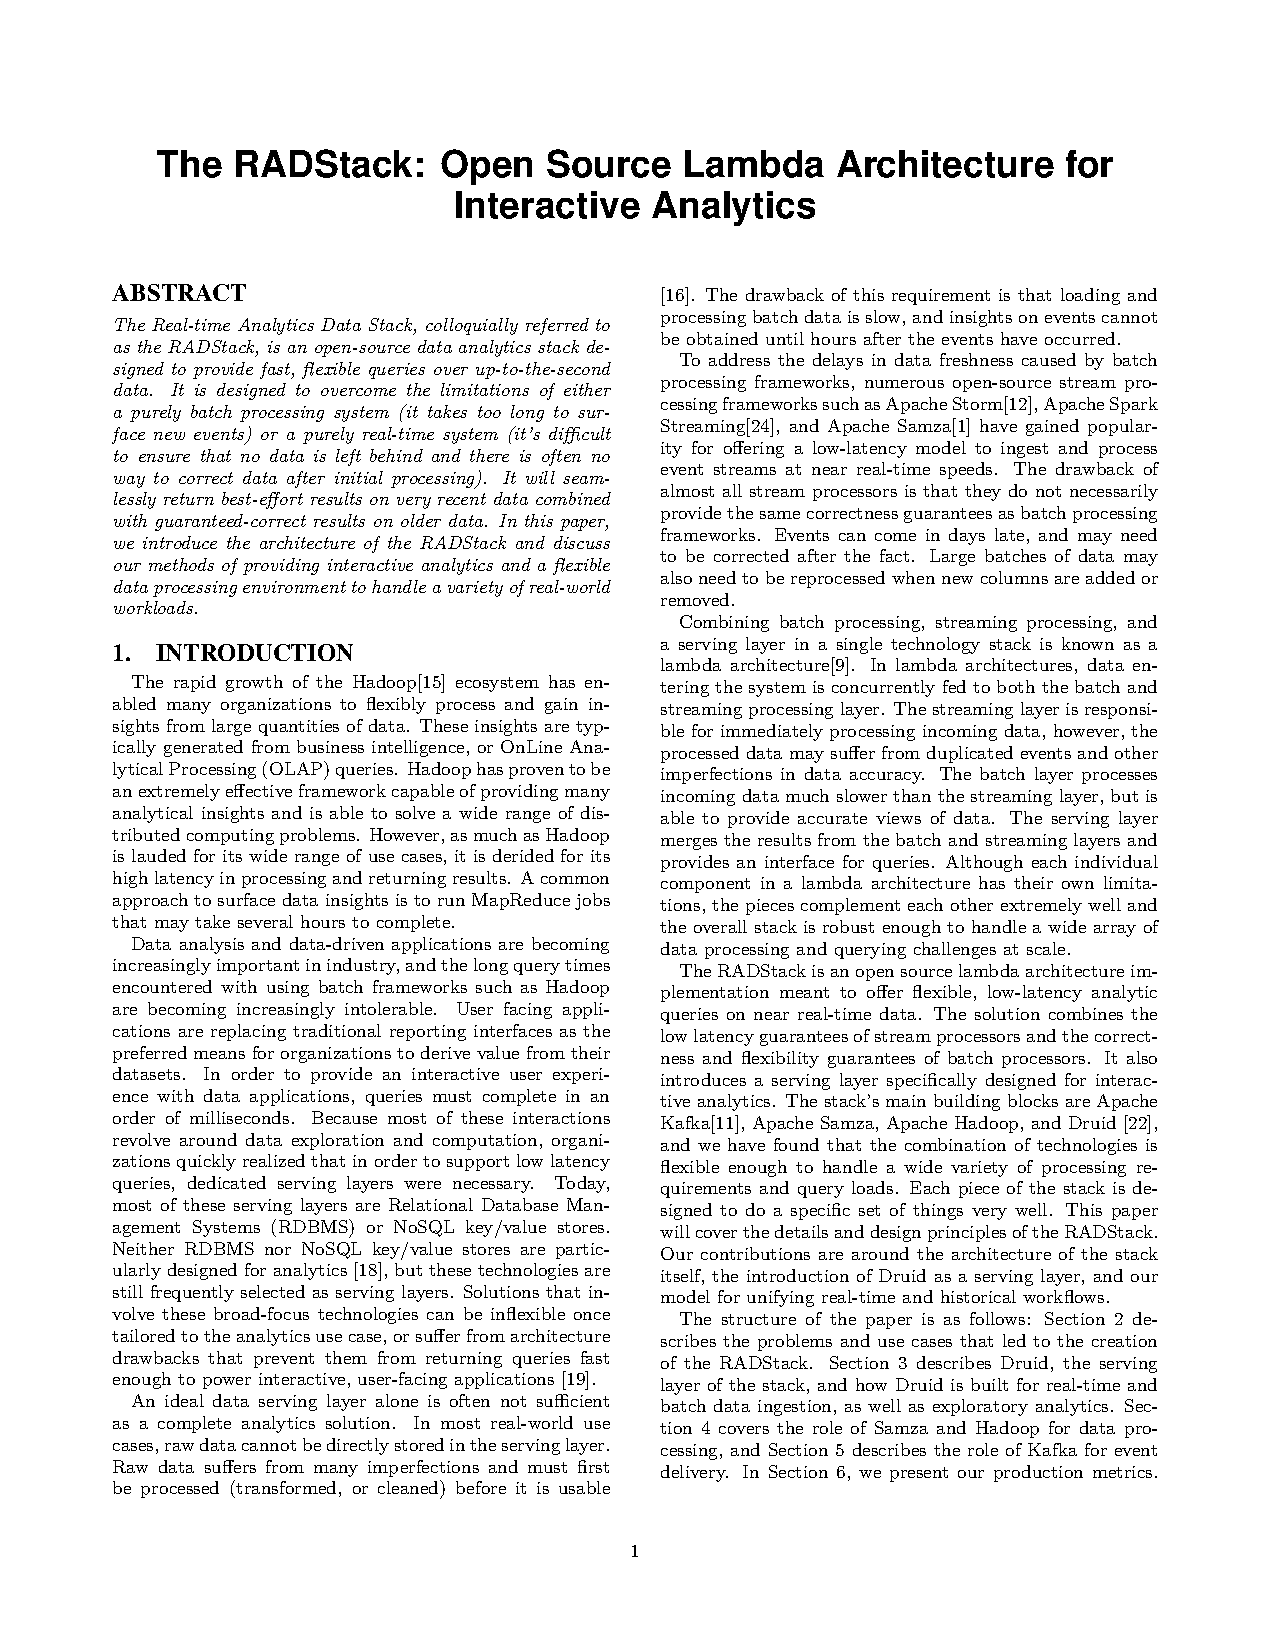
\includegraphics[width = 2.6in]{radstack}
\caption{
The components of the RADStack. Kafka acts as the event delivery
endpoints. Samza and Hadoop process data to load data into Druid. Druid acts as
the endpoint for queries.
}
\label{fig:radstack}
\end{figure}

To address these requirements of scale, stability, and performance, we created
Druid. Druid was designed from the ground up to provide arbitrary data
exploration, low latency aggregations, and fast data ingestion.  Druid was also
designed to accept fully denormalized data, and moves away from the traditional
relational model. Since most raw data is not denormalized, it must be processed
before it can be ingested and queried. Multiple streams of data had to be
joined, cleaned up, and transformed before it was usable in Druid, but that was
the trade-off we were willing to make in order to get the performance necessary
to power an interactive data application. We introduced stream processing to
our stack to provide the processing required before raw data could be loaded
into Druid. Our stream processing jobs range from simple data transformations,
such as id to name lookups, up to complex operations such as multi-stream
joins.  Pairing Druid with a stream processor enabled flexible data processing
and querying, but we still had problems with event delivery.  Our events were
delivered from many different locations and sources, and peaked at several
million events per second. We required a high throughput message bus that could
hold these events for consumpation by our stream processor.  To simplify data
transmission for our clients, we wanted the message bus to be the single
delivery endpoint for events entering our cluster.  

Our stack would be complete here if real-time processing were perfect, but the
open source stream processing space is still young. Processing jobs can go down
for extended periods of time and events may be delivered more than once.  These
are realities of any production data pipeline. To overcome these issues, we
included Hadoop in our stack to periodically clean up any data generated by the
real-time pipeline. We stored a copy of the raw events we received in a
distributed file system, and periodically ran batch processing jobs over this
data. The high level architecture of our setup is shown in Figure
~\ref{fig:radstack}. Each component is designed to do a specific set of things
well, and there is isolation in terms of functionality. Individual components
can entirely fail without impacting the services of the other components.

\begin{figure*}
\centering
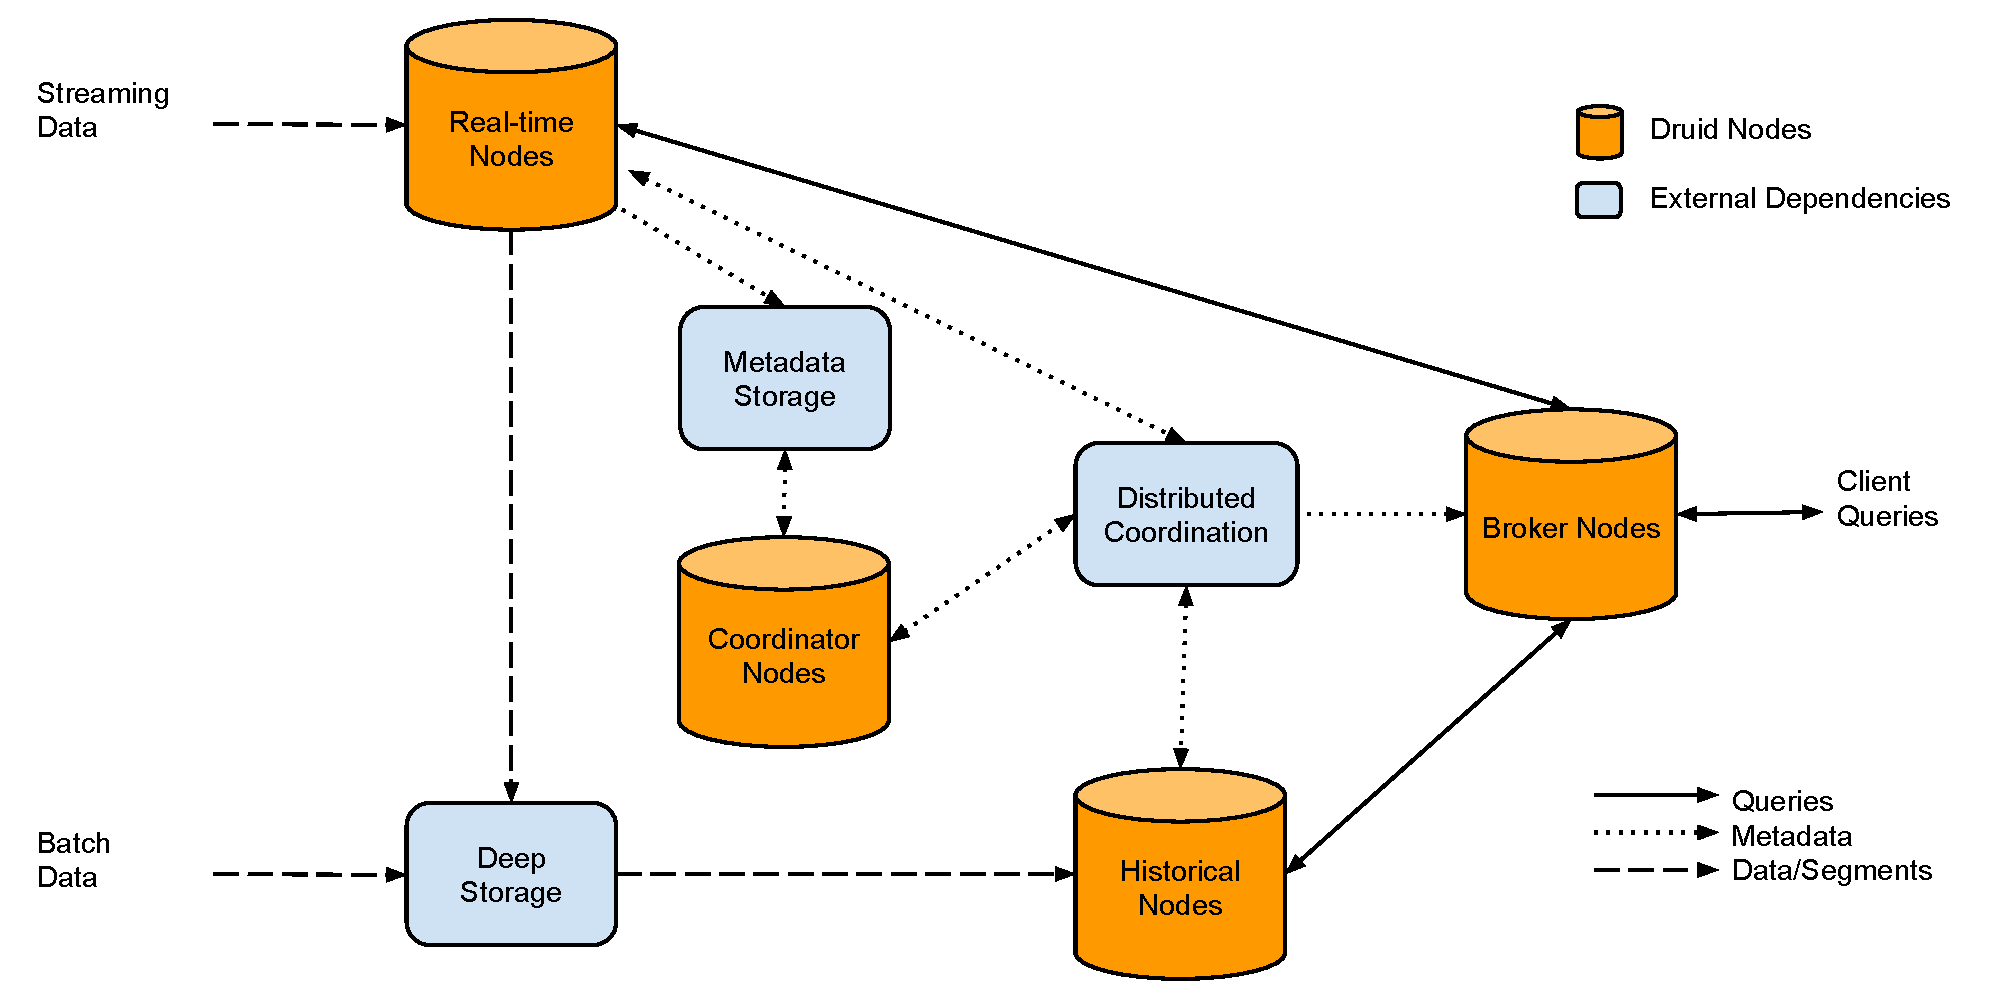
\includegraphics[width = 4.5in]{cluster}
\caption{An overview of a Druid cluster and the flow of data through the cluster.}
\label{fig:cluster}
\end{figure*}

\section{The Serving Layer}
\label{sec:serving}
Druid is a column-oriented data store designed for exploratory analytics and is
the serving layer in the RADStack. A Druid cluster consists of different types
of nodes and, similar to the overall design of the RADStack, each node type is
instrumented to perform a specific set of things well. We believe this design
separates concerns and simplifies the complexity of the overall system. To
solve complex data analysis problems, the different node types come together to
form a fully working system. The composition of and flow of data in a Druid
cluster are shown in Figure~\ref{fig:cluster}.

\subsection{Segments}
\label{sec:segments}
Data tables in Druid (called "data sources") are collections of timestamped
events and partitioned into a set of segments, where each segment is typically
5–10 million rows. Segments represent the fundamental storage unit in
Druid and Druid queries only understand how to scan segments. 

Druid always requires a timestamp column as a method of simplifying data
distribution policies, data retention policies, and first level query pruning.
Druid partitions its data sources into well defined time intervals, typically
an hour or a day, and may further partition on values from other columns to
achieve the desired segment size. The time granularity to partition segments is
a function of data volume and time range. A data set with timestamps spread
over a year is better partitioned by day, and a data set with timestamps spread
over a day is better partitioned by hour. 

Segments are uniquely identified by a data source identifier, the time interval
of the data, and a version string that increases whenever a new segment is
created. The version string indicates the freshness of segment data; segments
with later versions have newer views of data (over some time range) than
segments with older versions. This segment metadata is used by the system for
concurrency control; read operations always access data in a particular time
range from the segments with the latest version identifiers for that time
range.

Druid segments are stored in a column orientation. Given that Druid is best
used for aggregating event streams, the advantages of storing aggregate
information as columns rather than rows are well documented
\cite{abadi2008column}. Column storage allows for more efficient CPU usage as
only what is needed is actually loaded and scanned.  In a row oriented data
store, all columns associated with a row must be scanned as part of an
aggregation. The additional scan time can introduce significant performance
degradations \cite{abadi2008column}.

Druid nodes use one thread to scan one segment at a time, and the amount of
data that can be scanned in parallel is directly correlated to the number of
available cores in the cluster. Segments are immutable, and hence, this no
contention between reads and writes in a segment.

A single query may scan thousands of segments concurrently, and
many queries may run at the same time. We want to ensure that the entire
cluster is not starved out while a single expensive query is executing. Thus,
segments have an upper limit in how much data they can hold, and are sized
to be scanned in a few milliseconds. By keeping segment computation very fast,
cores and other resources are constantly being yielded. This ensures segments
from different queries are always being scanned.

Druid segments are very self-contained for the time interval of data that they
hold. Column data is stored directly in the segment. Druid has multiple column
types to represent various data formats. Timestamps are stored in long columns,
dimensions are stored in string columns, and metrics are stored in int, float,
long or double columns. Depending on the column type, different compression
methods may be used. Metric columns are compressed using
LZ4\cite{collet2013lz4} compression. String columns are dictionary encoded,
similar to other data stores such as PowerDrill\cite{hall2012processing}.
Additional indexes may be created for particular columns. For example, Druid
will by default create inverted indexes for string columns.

\subsection{Streaming Data Ingestion}
Druid real-time nodes encapsulate the functionality to ingest, query, and create
segments from event streams. Events indexed via these nodes are immediately
available for querying.  The nodes are only concerned with events for a relatively
small time range (e.g. hours) and periodically hand off immutable batches of events they
have collected over this small time range to other nodes in the Druid cluster
that are specialized in dealing with batches of immutable events. The nodes
announce their online state and the data they serve using a distributed
coordination service (this is currently Zookeeper\cite{hunt2010zookeeper}).

\begin{figure}
\centering
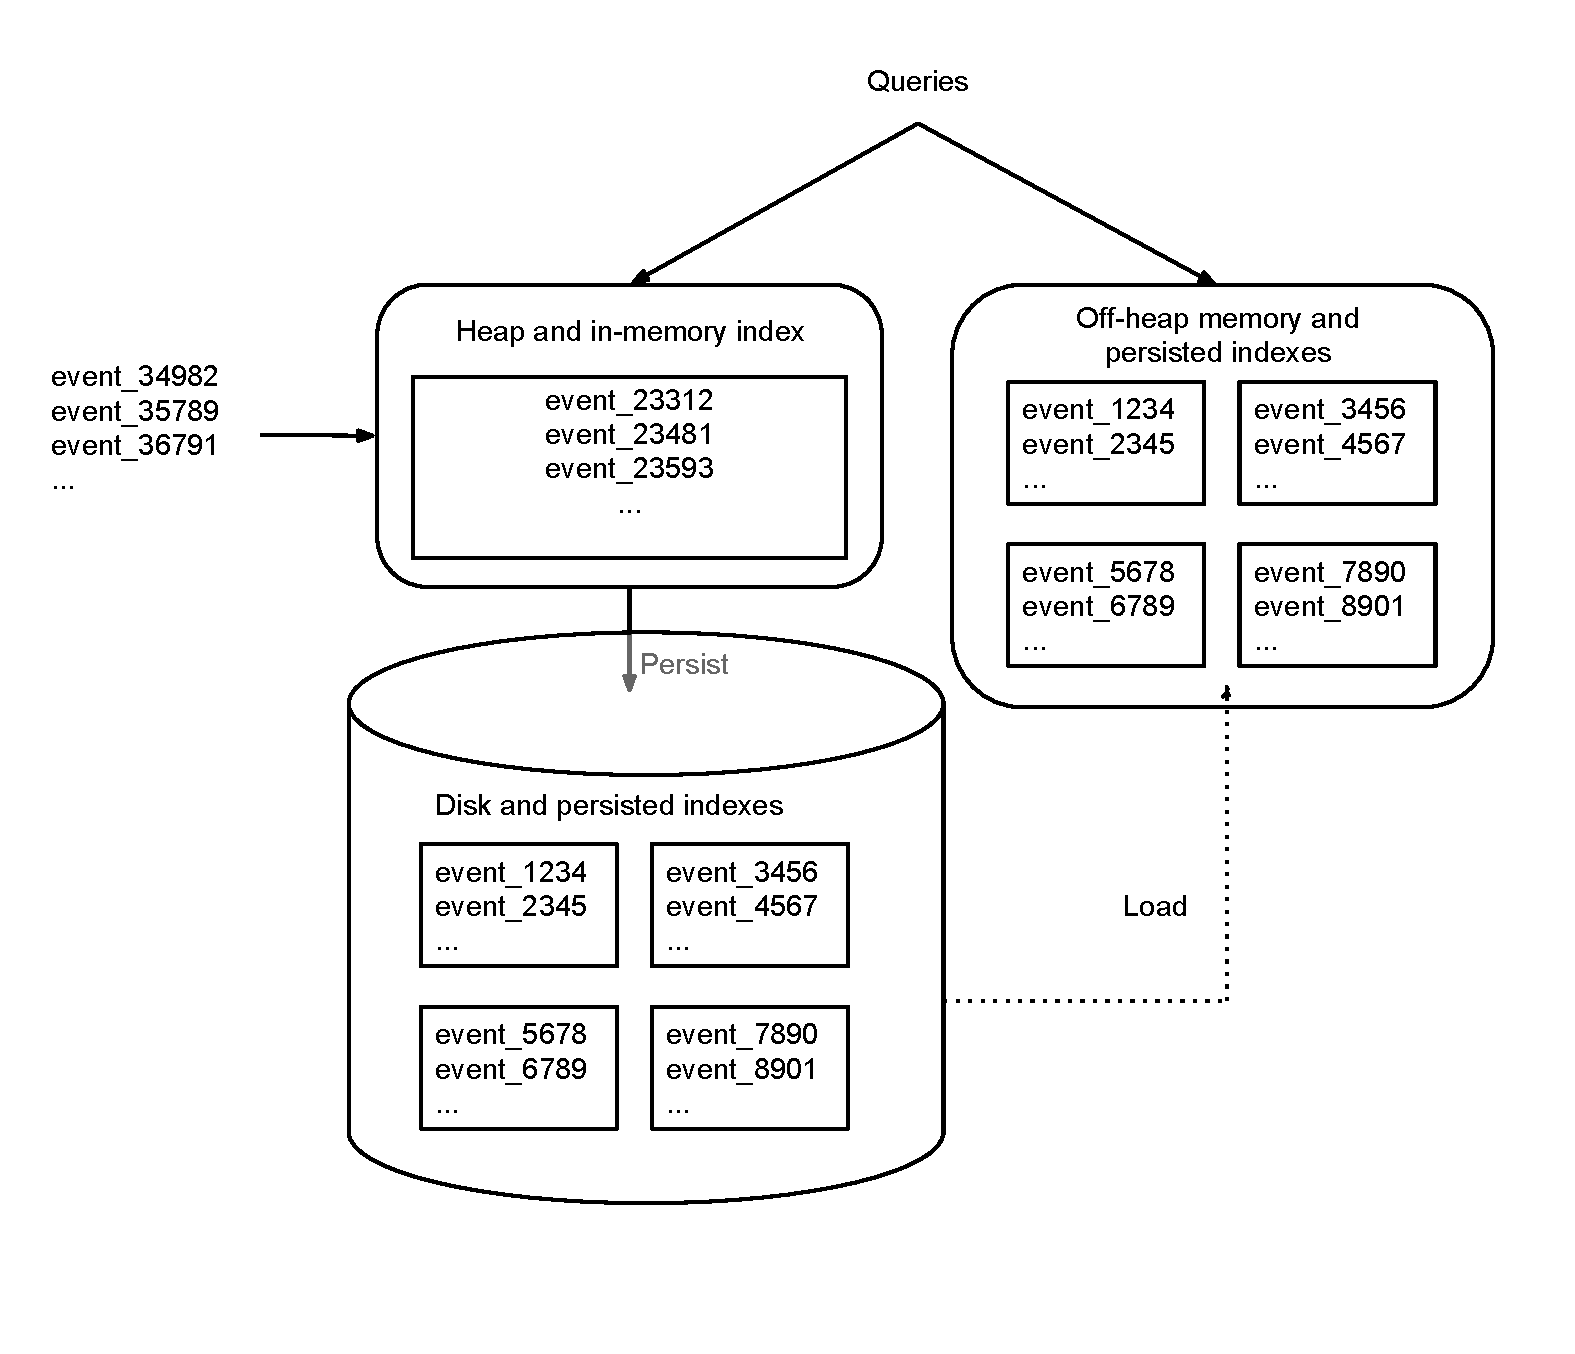
\includegraphics[width = 2.6in]{realtime_flow} 
\caption{
Real-time nodes write events to a write optimized in-memory index.
Periodically, events are persisted to disk, converting the write optimized
format to a read optimized one. On a periodic basis, persisted indexes are
then merged together and the final segment is handed off.  Queries will hit
both the in-memory and persisted indexes.  
}
\label{fig:realtime_flow}
\end{figure}

Real-time nodes employ a log structured merge tree\cite{o1996log} for recently
ingested data. Incoming events are first stored in an in-memory buffer. The
in-memory buffer is directly queryable and Druid behaves as a key/value store for
queries on events that exist in this JVM heap-based store. The in-memory buffer
is heavily write optimized, and given that Druid is really designed for heavy
concurrent reads, events do not remain in the in-memory buffer for very long.
Real-time nodes persist their in-memory indexes to disk either periodically or
after some maximum row limit is reached. This persist process converts data
stored in the in-memory buffer to the column oriented segment storage format
described in Section \ref{sec:segments}.  Persisted segments are memory mapped
and loaded to off-heap memory such that they can still be queried. This is
illustrated in Figure~\ref{fig:realtime_timeline}. Data is continuously
queryable during the persist process.

Real-time ingestion in Druid is self-throttling. If a significant spike occurs
in event volume from the upstream event producer, there are
a few safety mechanisms built in. Recall that events are first stored in an
in-memory buffer and persists can occur when a maximum configurable row limit
is reached. Spikes in event volume should cause persists to occur more often
and not overflow the in-memory buffer. However, the process of building a
segment does require time and resources. If too many concurrent persists occur,
and if events are added to the in-memory buffer faster than they can be removed
through the persist process, problems can still arise. Druid sets a limit on
the maximum number of persists that can occur at a time, and if this limit is
reached, Druid will begin to throttle event ingestion. In this case, the onus
is on the upstream consumer to be resilient in the face of increasing backlog.

Real-time nodes store recent data for a configurable period of time, typically
an hour. This period is referred to as the segment granularity period. The
nodes employ a sliding window to accept and reject events and use the
wall-clock time as the basis of the window. Events within a range of the node’s
wall-clock time are accepted, and events outside this window are dropped. This
period is referred to as the window period and typical window periods are 10
minutes in length. At the end of the segment granularity period plus the window
period, a real-time node will hand off the data it has collected during the
segment granularity period. The use of the window period means that delayed
events may be dropped. In practice, we see that these occurrences are rare, but
they do occur. Druid's real-time logic does not guarantee exactly once
processing and is instead best effort. The lack of exactly once processing in
Druid is one of the motivations for requiring batch fixup in the RADStack.

For further clarification, consider Figure~\ref{fig:realtime_timeline}.
Figure~\ref{fig:realtime_timeline} illustrates the operations of a real-time
node. The node starts at 13:37 and, with a 10 minute window period, will only
accept events for a window between 13:27 and 13:47.  When the first events are
ingested, the node announces that it is serving a segment for an
interval from 13:00 to 14:00. Every 10 minutes (the persist period is
configurable), the node will flush and persist its in-memory buffer to disk.
Near the end of the hour, the node will likely see events for 14:00 to 15:00.
When this occurs, the node prepares to serve data for the next hour and creates
a new in-memory buffer.  The node then announces that it is also serving a
segment from 14:00 to 15:00.  At 13:10, which is the end of the hour plus the
window period, the node begins the hand off process.

\begin{figure*}
\centering

\includegraphics[width = 4.5in]{realtime_timeline}
\caption{The node starts, ingests data, persists, and periodically hands data
off. This process repeats indefinitely. The time periods between different
real-time node operations are configurable.}
\label{fig:realtime_timeline}
\end{figure*}

\subsection{Hand off}
Real-time nodes are designed to deal with a small window of recent data and
need periodically hand off segments they’ve built. The hand-off process first
involves a compaction step. The compaction process finds all the segments that
were created for a specific interval of time (for example, all the segments
that were created by intermediate persists over the period of an hour). These
segments are merged together to form a final immutable segment for handoff. 

Handoff occurs in a few steps. First, the finalized segment is uploaded to a
permanent backup storage, typically a distributed file system such as S3
\cite{decandia2007dynamo} or HDFS \cite{shvachko2010hadoop}, which Druid refers
to as “deep storage”. Next, an entry is created in the metadata store
(typically a RDBMS such as MySQL) to indicate that a new segment has been
created. This entry in the metadata store will eventually cause other nodes in
the Druid cluster to download and serve the segment. The real-time node
continues to serve the segment until it notices that the segment is available
on Druid historical nodes, which are nodes that are dedicated to serving
historical data. At this point, the segment is dropped and unannounced from the
real-time node. The entire handoff process is fluid; data remains continuously
queryable throughout the entire handoff process. Segments created by real-time
processing are versioned by the start of the segment granularity interval.

\subsection{Batch Data Ingestion}
The core component used by real-time ingestion is a hash map that can be
incrementally populated and finalized to create an immutable segment. This core
component is shared across both real-time and batch ingestion. Druid has built
in support for creating segments by leveraging Hadoop and running MapReduce
jobs to partition data for segments.  Events can be read in one at a time
directly from static files in a "streaming" fashion.

Similar to the real-time ingestion logic, segments created through batch
ingestion are directly uploaded to deep storage. Druid’s Hadoop-based batch
indexer will also create an entry in the metadata storage once all segments
have been created. The version of the segments created by batch ingestion are
based on the time the batch processing job started at.

\subsection{Unifying Views}
When new entries are created in the metadata storage, they will eventually be
noticed by Druid coordinator nodes. Druid coordinator nodes poll the metadata
storage for what segments should be loaded on Druid historical nodes, and
compare the result with what is actually loaded on those nodes. Coordinator
nodes will tell historical nodes to load new segments, drop outdated segments,
and move segments across nodes.

Druid historical nodes are very simple in operation. They know how to load,
drop, and respond to queries to scan segments. Historical nodes typically
store all the data that is older than an hour (recent data lives on the
real-time node). The real-time handoff process requires that a historical must
first load and begin serving queries for a segment before that segment can
be dropped from the real-time node. Since segments are immutable, the same copy
of a segment can exist on multiple historical nodes and real-time nodes. Most
nodes in typical production Druid clusters are historical nodes.

To consolidate results from historical and real-time nodes, Druid has a set of
broker nodes which act as the client query endpoint. Broker nodes in part
function as query routers to historical and real-time nodes. Broker nodes
understand the metadata published in distributed coordination service
(Zookeeper) about what segments are queryable and where those segments are
located. Broker nodes route incoming queries such that the queries hit the
right historical or real-time nodes.  Broker nodes also merge partial results
from historical and real-time nodes before returning a final consolidated
result to the caller.

Broker nodes maintain a segment timeline containing information about what
segments exist in the cluster and the version of those segments. Druid uses
multi-version concuncurrency control to manage how data is extracted from
segments. Segments with higher version identifiers have precedence over
segments with lower version identifiers. If two segments exactly overlap for an
interval, Druid only considers the data from the segment with the higher
version. This is illustrated in Figure~\ref{fig:timeline}

\begin{figure}
\centering
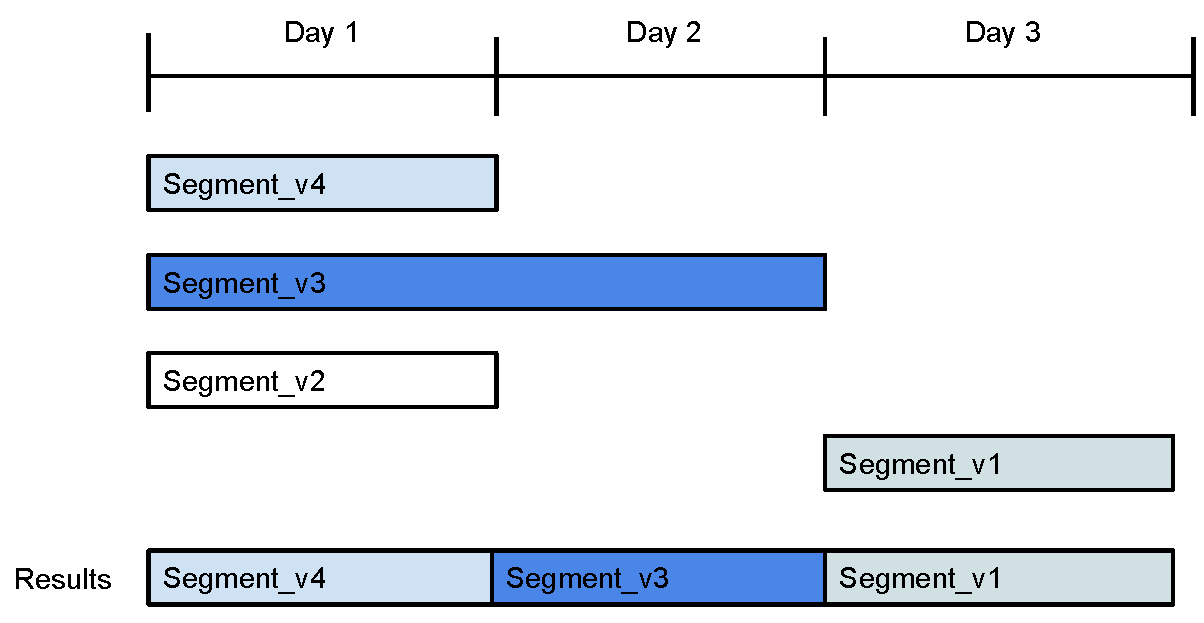
\includegraphics[width = 2.6in]{timeline}
\caption{
Druid utilizes multi-version concurrency control and reads data from segments
with the latest version for a given interval. Segments that are that completely
overshadowed are ignored and eventually automatically dropped from the cluster.
}
\label{fig:timeline}
\end{figure}

Segments are inserted into the timeline as they are announced. The timeline
sorts the segment based on their data interval in a data structure similar to
an interval tree. Lookups in the timeline will return all segments with
intervals that overlap the lookup interval, along with interval ranges for
which the data in a segment is valid. 

Brokers extract the interval of a query and use it for lookups into the
timeline. The result of the timeline is used to remap the original query into a
set of specific queries for the actual historical and real-time nodes that hold
the pertinent query data. The results from the historical and real-time nodes
are finally merged by the broker, which returns the final result to the caller.

The coordinator node also builds a segment timeline for segments in the
cluster. If a segment is completely overshadowed by one or more segments, it
will be flagged in this timeline. When the coordinator notices overshadowed
segments, it tells historical nodes to drop these segments from the cluster.

\section{The Processing Layer}
\label{sec:processing}
Although Druid can ingest events that are streamed in one at a time, data must
be denormalized beforehand as Druid cannot yet support
join queries. Furthermore, real world data must often be transformed before it
is usable by an application.

\subsection{Stream Processing}
\label{sec:streamprocessing}
Stream processors provide infrastructure to develop processing logic for
unbounded sequences of messages. We use Apache Samza as our stream processor,
although other technologies are viable alternatives (we initially chose Storm,
but have since switched to Samza). Samza provides an API to write jobs that run
over a sequence of tuples and perform operations over those tuples in a
user-defined way. The input to each job is provided by Kafka, which can also
act as a sink for the output of the job. Samza jobs are executed in a resource
management and task execution framework such as
YARN\cite{vavilapalli2013apache}. It is beyond the scope of this paper to go
into the full details of Kafka/YARN/Samza interactions, but more information is
available in other literature\cite{2014samza}. We will instead focus on how we
leverage this framework for processing data for analytic use cases.

On top of Samza infrastructure, we introduce the idea of a “pipeline”, which is
a grouping for a series of related processing stages where “upstream” stages
produce messages that are consumed by “downstream” stages. Some of our jobs
involve operations such as renaming data, inserting default values for nulls
and empty strings, and filtering data. One pipeline may write to many data
sources in Druid.

To understand a real-world pipeline, let's consider an example from online
advertising. In online advertising, events are generated by impressions (views)
of an ad and clicks of an ad. Many advertisers are interested in knowing how
many impressions of an ad converted into clicks. Impression streams and click
streams are almost always generated as separate streams by ad servers. Recall
that Druid does not support joins at query time, so the events must be
generated at processing time. An example of data generated by these two event
streams is shown in Figure~\ref{fig:imps_clicks}. Every event has a unique
impression id that identifies the ad served. We use this id as our join key.

\begin{figure}
\centering
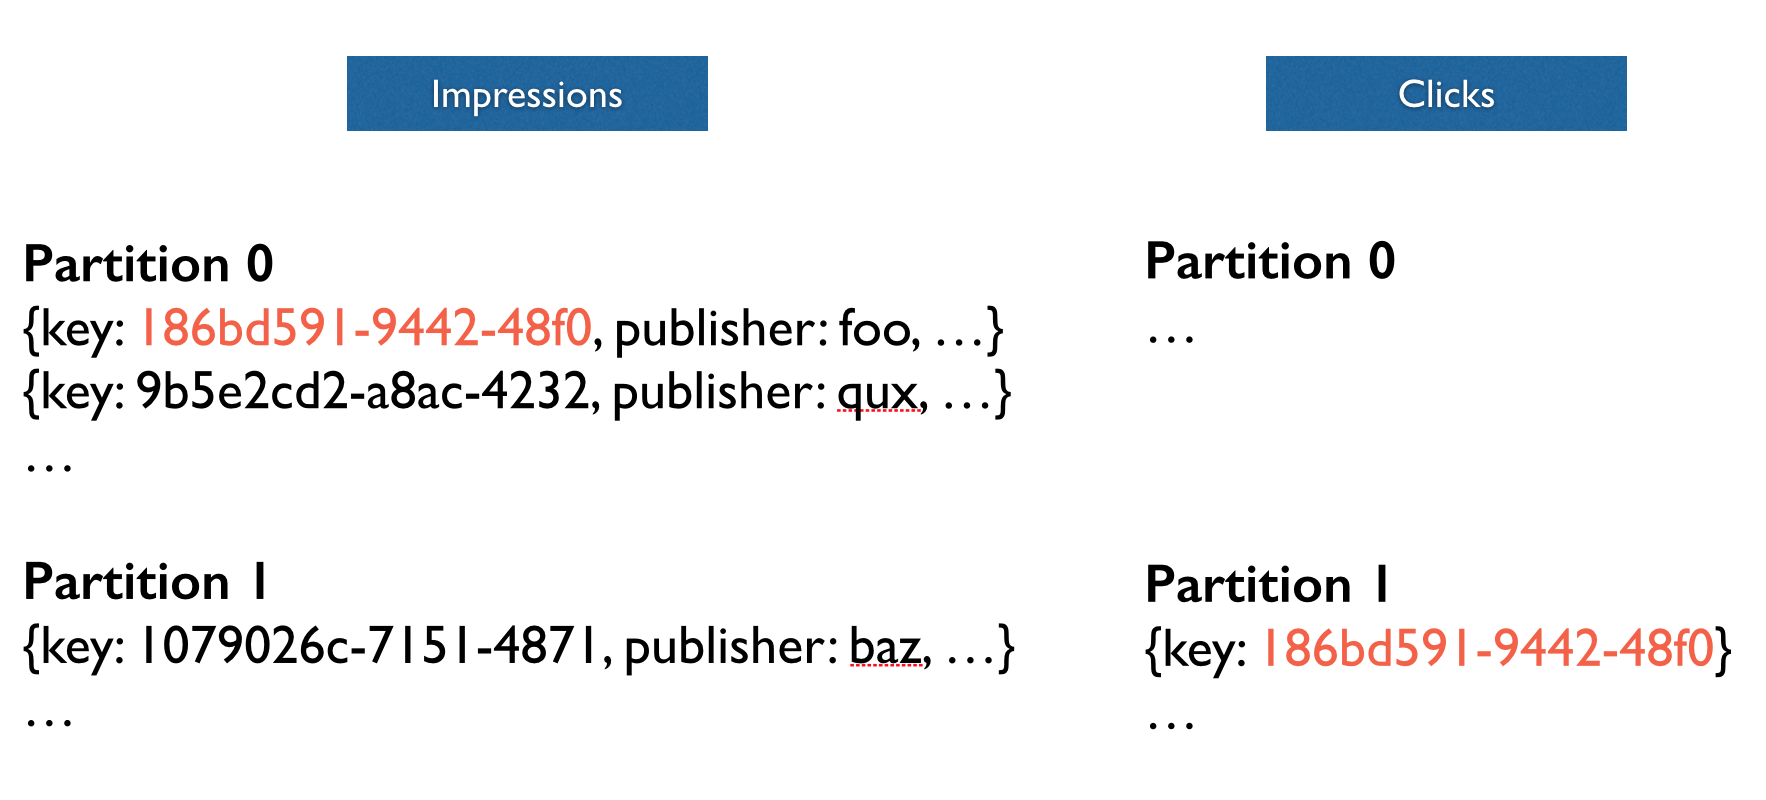
\includegraphics[width = 2.6in]{imps_clicks} 
\caption{ 
Ad impressions
and clicks are recorded in two separate streams. An event we want to join is
located in two different Kafka partitions on two different topics.  
}
\label{fig:imps_clicks}
\end{figure}

The first stage of the Samza processing pipeline is a shuffle step. Events are
written to a keyed Kafka topic based on the hash of an event's impression id.
This ensures that the events that need to be joined are written to the same
Kafka topic. YARN containers running Samza tasks may read from one or more
Kafka topics, so it is important Samza task for joins actually has both events
that need to be joined. This is shuffle stage is shown in
Figure~\ref{fig:shuffled}.

\begin{figure}
\centering
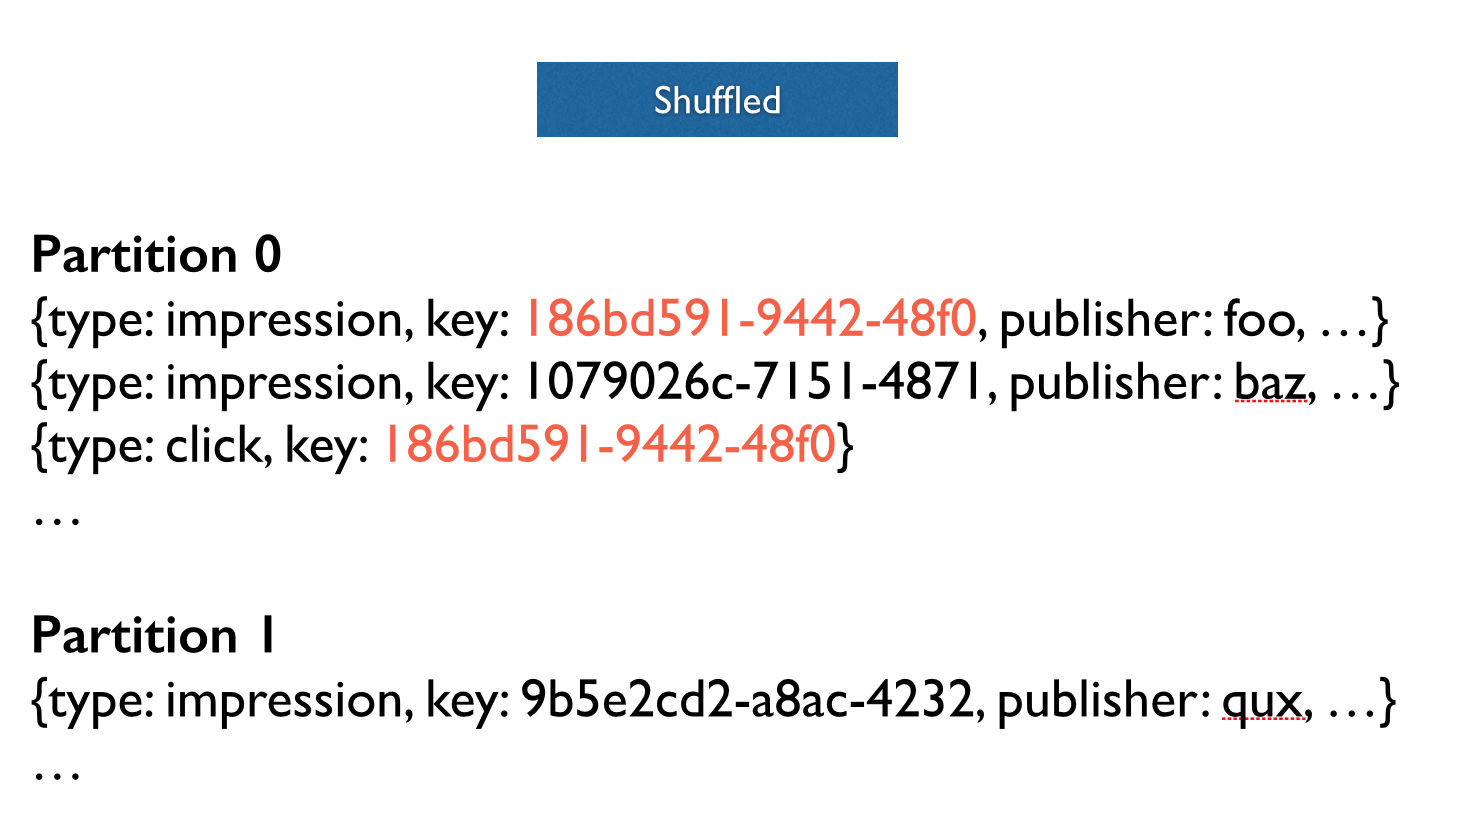
\includegraphics[width = 2.6in]{shuffled}
\caption{
A shuffle operation ensures events to be joined at stored in the same Kafka
partition.
}
\label{fig:shuffled}
\end{figure}

The next stage in the data pipeline is to actually join the impression and
click events. This is done by another Samza task that creates a new event in
the data with a new field called "is\_clicked".  This field is marked as "true"
if an impression event and a click event with the same impression id are both
present. The original events are discarded, and the new event is send further
downstream. This join stage shown in Figure~\ref{fig:joined}

\begin{figure}
\centering
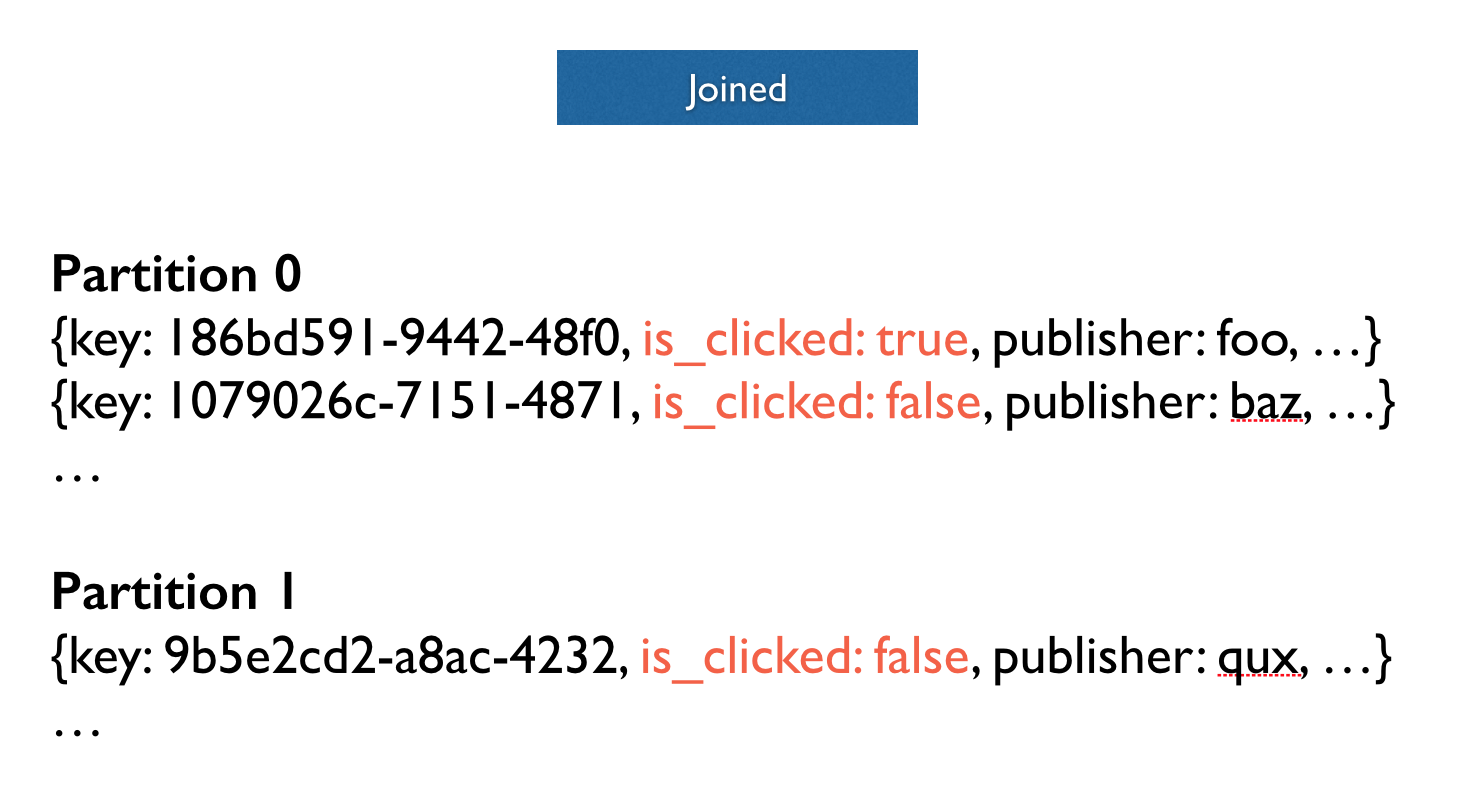
\includegraphics[width = 2.6in]{joined}
\caption{
The join operation adds a new field, "is\_clicked".
}
\label{fig:joined}
\end{figure}

The final stage of our data processing is to enhance the data. This stage
cleans up faults in data, and performs lookups and transforms of events. Once
data is cleaned, it is ready to be delivered to Druid for queries. The total
streaming data processing pipeline is shown in Figure~\ref{fig:pipeline}.

\begin{figure}
\centering
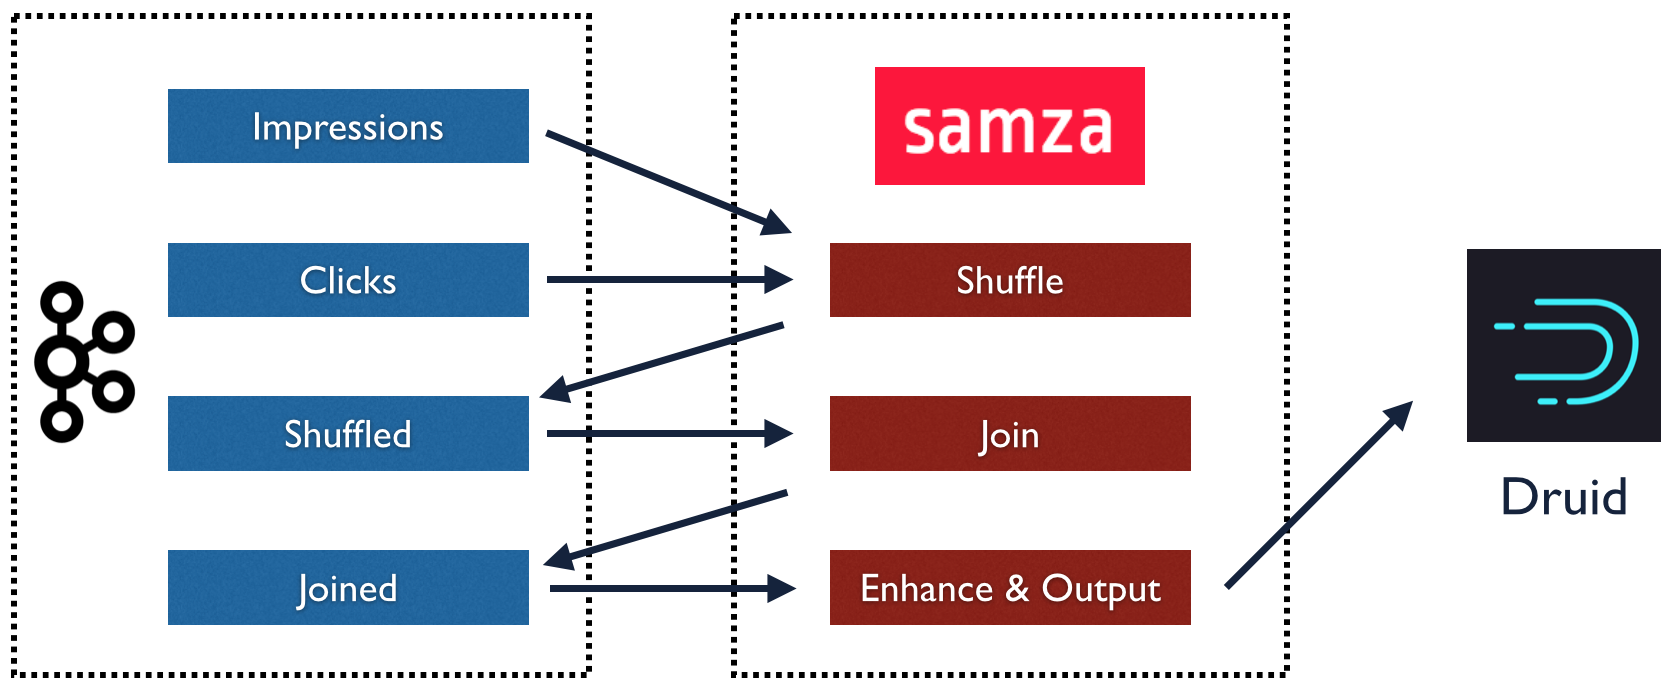
\includegraphics[width = 2.6in]{pipeline}
\caption{
The streaming processing data pipeline.
}
\label{fig:pipeline}
\end{figure}

The system we have designed is not perfect. Because we are doing windowed joins
and because events cannot be buffered indefinitely, not all joins are
guaranteed to complete. If events are substantially delayed and do not arrive
in the allocated window period, they will not be joined. In practice, this
generally leads to one “primary” event continuing through the pipeline and
other secondary events with the same join key getting dropped.  This means that
our stream processing layer is not guaranteed to deliver 100\% accurate
results. Furthermore, even without this restriction, Samza does not offer
exactly-once processing semantics. Problems in network connectivity or node
failure can lead to duplicated events. For these reasons, we run a separate
batch pipeline that generates a more accurate transformation of the ingested
data.

The final job of our processing pipeline is to deliver data to Druid. For high
availability, processed events from Samza are transmitted concurrently to two
real-time nodes. Both nodes receive the same copy of data, and effectively act
as replicas of each other. The Druid broker can query for either copy of the data.
When handoff occurs, both real-time nodes race to hand off the segments they’ve
created. The segment that is pushed into deep storage first will be the one
that is used for historical querying, and once that segment is loaded on the
historical nodes, both real-time nodes will drop their versions of the same
segment.

\subsection{Batch Processing}
Our batch processing pipeline is composed of a multi-stage
MapReduce\cite{dean2008mapreduce} pipeline. The first set of jobs mirrors our
stream processing pipeline in that it transforms data and joins relevant events
in preparation for the data to be loaded into Druid. The second set of jobs is
responsible for directly creating immutable Druid segments. The indexing code
for both streaming and batch ingestion in Druid is shared between the two modes
of ingestion. These segments are then uploaded to deep storage and registered
with the metadata store. Druid will proceed to load the batch generated
segments.

The batch process typically runs much less frequently than the real-time
process, and may run many hours or even days after raw events have been
delivered. The wait is necessary for severely delayed events, and to ensure
that the raw data is indeed complete. 

Segments generated by the batch process are versioned by the start time of the
process. Hence, segments created by batch processing will have a version
identifier that is greater than segments created by real-time processing. When
these batch created segments are loaded in the cluster, they atomically replace
segments created by real-time processing for their processed interval. Hence,
soon after batch processing completes, Druid queries begin reflecting
batch-originated data rather than real-time-originated data.

We use the streaming data pipeline described in
Section\ref{sec:streamprocessing} to deliver immediate insights on events as
they are occurring, and the batch data pipeline described in this section to
provide an accurate copy of the data. The batch process typically runs much
less frequently than the real-time process, and may run many hours or even days
after raw events have been delivered. The wait is necessary for severely
delayed events, and to ensure that the raw data is indeed complete. 

\section{The Delivery Layer}
\label{sec:delivery}
In our stack, events are delivered over HTTP to Kafka. Events are transmitted
via POST requests to a receiver that acts as a front for a Kafka producer.
Kafka is a distributed messaging system with a publish and subscribe model. At
a high level, Kafka maintains events or messages in categories called topics. A
distributed Kafka cluster consists of numerous brokers, which store messages in
a replicated commit log. Kafka consumers subscribe to topics and process feeds
of published messages. 

Kafka provides functionality isolation between producers of data and consumers
of data. The publish/subscribe model works well for our use case as multiple
consumers can subscribe to the same topic and process the same set of events.
We have two primary Kafka consumers. The first is a Samza job that reads
messages from Kafka for stream processing as described in Section
\ref{sec:streamprocessing}. Topics in Kafka map to pipelines in Samza, and
pipelines in Samza map to data sources in Druid. The second consumer reads
messages from Kafka and stores them in a distributed file system.  This file
system is the same as the one used for Druid’s deep storage, and also acts as a
backup for raw events. The purpose of storing raw events in deep storage is so
that we can run batch processing jobs over them at any given time. For example,
our stream processing layer may choose to not include certain columns when it
first processes a new pipeline. If we want to include these columns in the
future, we can reprocess the raw data to generate new Druid segments. 

Kafka is the single point of delivery for events entering our system, and must
have the highest availability. We replicate our Kafka producers across multiple
datacenters. In the event that Kafka brokers and consumers become unresponsive,
as long as our HTTP endpoints are still available, we can buffer events on the
producer side while recovering the system. Similarily, if our processing and
serving layers completely fail, we can recover by replaying events from Kafka.

\section{Performance}
\label{sec:performance}
Druid runs in production at several organizations, and to briefly demonstrate
its performance, we have chosen to share some real world numbers for one of the larger
production clusters. We also include results from synthetic workloads on TPC-H data.

\subsection{Query Performance in Production}
Druid query performance can vary signficantly depending on the query being
issued. For example, sorting the values of a high cardinality dimension based
on a given metric is much more expensive than a simple count over a time range.
To showcase the average query latencies in a production Druid cluster, we
selected 8 of our most queried data sources, described in
Table~\ref{tab:datasources}.

\begin{table}
  \centering
  \scriptsize\begin{tabular}{| l | l | l |}
    \hline
    \textbf{Data Source} & \textbf{Dimensions} & \textbf{Metrics} \\ \hline
    \texttt{a} & 25 & 21 \\ \hline
    \texttt{b} & 30 & 26 \\ \hline
    \texttt{c} & 71 & 35 \\ \hline
    \texttt{d} & 60 & 19 \\ \hline
    \texttt{e} & 29 & 8 \\ \hline
    \texttt{f} & 30 & 16 \\ \hline
    \texttt{g} & 26 & 18 \\ \hline
    \texttt{h} & 78 & 14 \\ \hline
  \end{tabular}
  \normalsize
  \caption{Characteristics of production data sources.}
  \label{tab:datasources}
\end{table}

Approximately 30\% of queries are standard aggregates involving different types
of metrics and filters, 60\% of queries are ordered group bys over one or more
dimensions with aggregates, and 10\% of queries are search queries and metadata
retrieval queries. The number of columns scanned in aggregate queries roughly
follows an exponential distribution. Queries involving a single column are very
frequent, and queries involving all columns are very rare.

\begin{itemize}[leftmargin=*,beginpenalty=5000,topsep=0pt]
\item There were
approximately 50 total data sources in this particular cluster and several hundred users issuing
queries.

\item There was approximately 10.5TB of RAM available in this cluster and
approximately 10TB of segments loaded. Collectively,
there are about 50 billion Druid rows in this cluster. Results for
every data source is not shown.

\item This cluster uses Intel\textsuperscript{\textregistered} Xeon\textsuperscript{\textregistered} E5-2670 processors and consists of 1302 processing
threads and 672 total cores (hyperthreaded).

\item A memory-mapped storage engine was used (the machine was configured to
    memory map the data instead of loading it into the Java heap.)
\end{itemize}

Query latencies are shown in Figure~\ref{fig:query_latency}. Across all the various
data sources, average query latency is approximately 550 milliseconds, with
90\% of queries returning in less than 1 second, 95\% in under 2 seconds, and
99\% of queries returning in less than 10 seconds. Occasionally we observe
spikes in latency, as observed on February 19, where network issues on
the broker nodes were compounded by very high query load on one of our
largest data sources.

\subsection{Query Benchmarks on TPC-H Data}
We also present Druid benchmarks on TPC-H data.  Most TPC-H queries do not
directly apply to Druid, so we selected queries more typical of Druid's
workload to demonstrate query performance. In Figure~\ref{fig:tpch_scaling}, we
present our results of scaling Druid to meet increasing data volumes with the
TPC-H 100 GB data set. We observe that when we increased the number of cores
from 8 to 48, not all types of queries achieve linear scaling, but the simpler
aggregation queries do. The increase in speed of a parallel computing system is
often limited by the time needed for the sequential operations of the system.
In this case, queries requiring a substantial amount of work at the broker
level do not parallelize as well.

\begin{figure}
\centering
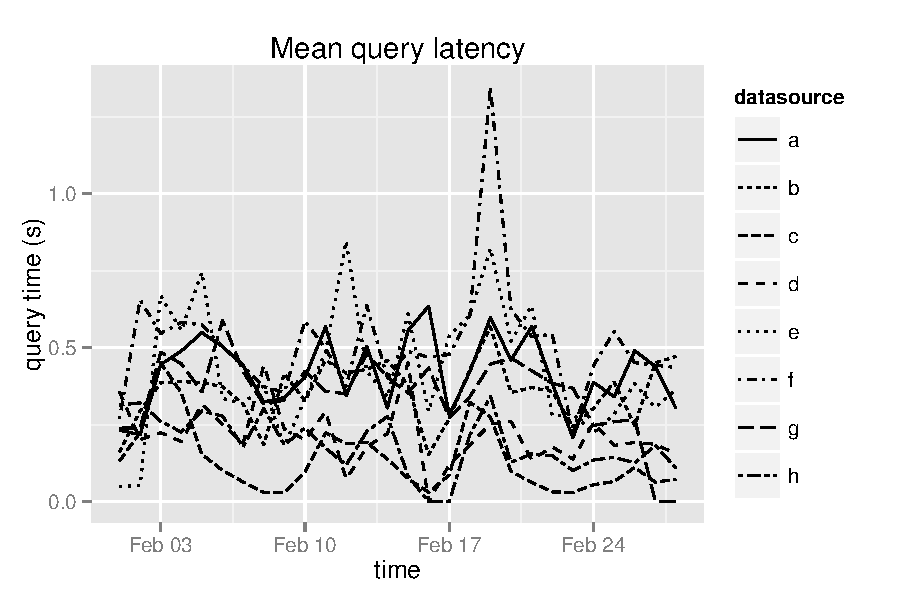
\includegraphics[width = 2.3in]{avg_query_latency}
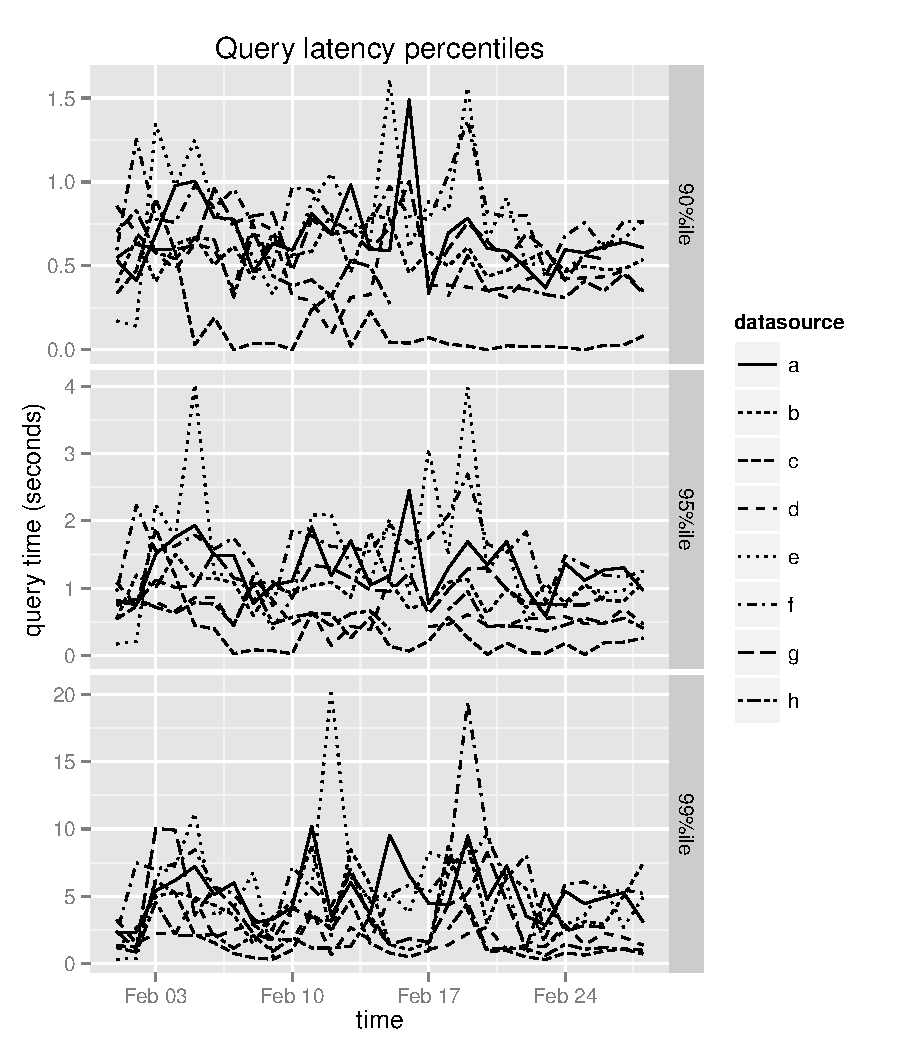
\includegraphics[width = 2.3in]{query_percentiles}
\caption{Query latencies of production data sources.}
\label{fig:query_latency}
\end{figure}

\begin{figure}
\centering
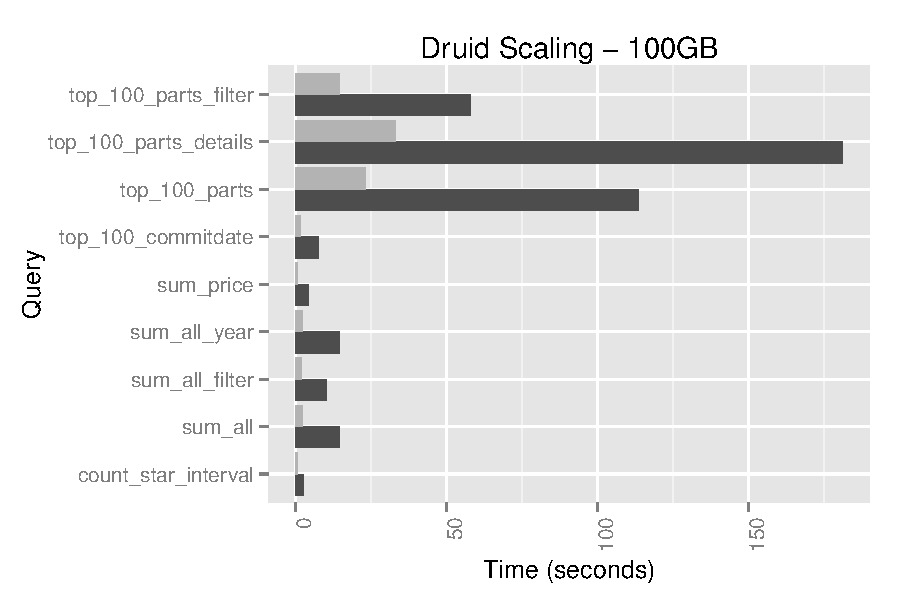
\includegraphics[width = 2.3in]{tpch_scaling}
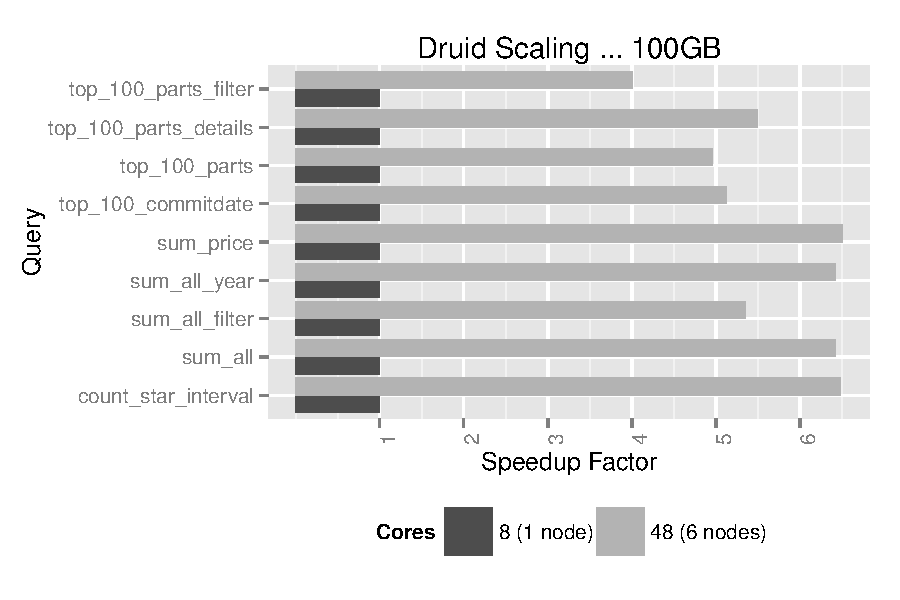
\includegraphics[width = 2.3in]{tpch_scaling_factor}
\caption{Druid scaling benchmarks -- 100GB TPC-H data.}
\label{fig:tpch_scaling}
\end{figure}

Our Druid setup used Amazon EC2 \texttt{m3.2xlarge} instance types
(Intel\textsuperscript{\textregistered} Xeon\textsuperscript{\textregistered}
E5-2680 v2 @ 2.80GHz) for historical nodes and \texttt{c3.2xlarge} instances
(Intel\textsuperscript{\textregistered} Xeon\textsuperscript{\textregistered}
E5-2670 v2 @ 2.50GHz) for broker nodes. 

We benchmarked Druid's scan rate at 53,539,211
rows/second/core for \texttt{select count(*)} equivalent query over a given
time interval and 36,246,530 rows/second/core for a \texttt{select sum(float)}
type query.

\subsection{Data Ingestion Performance}
To showcase the ingestion latency of the RADStack, we selected the top seven
production datasources in terms of peak events ingested per second for early
2015. These datasources are described in Table~\ref{tab:ingestion}. Our
production ingestion setup used over 40 nodes, each with 60GB of RAM and 32
cores (12 x Intel\textsuperscript\textregistered
Xeon\textsuperscript\textregistered E5-2670). In this setup, many other Druid
related ingestion tasks were running concurrently on the machines. Each
pipeline for each datasource involved transforms and joins.

\begin{table}
  \centering
  \scriptsize\begin{tabular}{| l | l | l | l |}
    \hline
    \textbf{Data Source} & \textbf{Dimensions} & \textbf{Metrics} & \textbf{Peak Events/s} \\ \hline
    \texttt{d1} & 34 & 24 & 218123 \\ \hline
    \texttt{d2} & 36 & 24 & 172902 \\ \hline
    \texttt{d3} & 46 & 21 & 170264 \\ \hline
    \texttt{d4} & 40 & 17 & 94064 \\ \hline
    \texttt{d5} & 41 & 23 & 68104 \\ \hline
    \texttt{d6} & 31 & 31 & 64222 \\ \hline
    \texttt{d7} & 29 & 8 & 30048 \\ \hline
  \end{tabular}
  \normalsize
  \caption{Characteristics of production data sources.}
  \label{tab:ingestion}
\end{table}

Ingestion latency is heavily dependent on the complexity of the data set being
ingested. The data complexity is determined by the number of dimensions in each
event, the number of metrics in each event, and the types of aggregations we
want to perform on those metrics. With the most basic data set (one that only
has a timestamp column), our setup can ingest data at a rate of 800,000
events/second/core, which is really just a measurement of how fast we can
deserialize events. At peak, a single node was able to process 62259
events/second. The total peak events per second was
840500. The median events per second was 590100. The first and third quantiles
were 487000 events/s and 663200 events/s respectively. 

\section{Production Experiences}
\label{sec:experiences}

\subsection{Experiences with Druid}
\subsubsection{Query Patterns}
Druid is often used for exploratory analytics and reporting, which are two very
distinct use cases. Exploratory analytic workflows provide insights by
progressively narrowing down a view of data until an interesting observation is
made. Users tend to explore short intervals of recent data. In the reporting
use case, users query for much longer data intervals, and the volume of queries
is generally much less. The insights that users are looking for are often
pre-determined. 

\subsubsection{Multitenancy}
Expensive concurrent queries can be problematic in a multitenant environment.
Queries for large data sources may end up hitting every historical node in a
cluster and consume all cluster resources. Smaller, cheaper queries may be
blocked from executing in such cases. We introduced query prioritization to
address these issues. Each historical node is able to prioritize which segments
it needs to scan. Proper query planning is critical for production workloads.
Thankfully, queries for a significant amount of data tend to be for reporting
use cases and can be de-prioritized. Users do not expect the same level of
interactivity in this use case as they do when they are exploring data. 

\subsubsection{Node Failures}
Single node failures are common in distributed environments, but many nodes
failing at once are not. If historical nodes completely fail and do not
recover, their segments need to be reassigned, which means we need excess
cluster capacity to load this data. The amount of additional capacity to have
at any time contributes to the cost of running a cluster. From our experiences,
it is extremely rare to see more than 2 nodes completely fail at once and
hence, we leave enough capacity in our cluster to completely reassign the data
from 2 historical nodes. 

\subsection{Experiences with Ingestion}
\subsubsection{Multitenancy}
Before moving our streaming pipeline to Samza, we experimented with other
stream processors. One of the biggest pains we felt was around multi-tenancy. Multiple
pipelines may contend for resources, and it is often unclear how various jobs
impact one another when running in the same environment. Given that each of our
pipelines is composed of different tasks, Samza was able to provide per task
resource isolation, which was far easier to manage than per application
resource isolation.

\subsection{Operational Monitoring}
Proper monitoring is critical to run a large scale distributed cluster,
especially with many different technologies. Each Druid node is designed to
periodically emit a set of operational metrics. These metrics may include
system level data such as CPU usage, available memory, and disk capacity, JVM
statistics such as garbage collection time, and heap usage, or node specific
metrics such as segment scan time, cache hit rates, and data ingestion
latencies. Druid also emits per query metrics so we can examine why a
particular query may be slow. We’ve also added functionality to periodically
emit metrics from Samza, Kafka, and Hadoop. We emit metrics from our production
RADStack and load them into a dedicated metrics RADstack. The metrics cluster
is used to explore the performance and stability of the production cluster.
This dedicated metrics cluster has allowed us to find numerous production
problems, such as gradual query speed degradations, less than optimally tuned
hardware, and various other system bottlenecks.

\section{Related Work}
\label{sec:related}

\subsection{Hybrid Batch/Streaming Workflows}

Spark\cite{zaharia2012resilient} is a cluster computing framework optimized for
iterative workflows.  Spark Streaming is a separate project that converts
sequences of tuples into immutable micro-batches. Each micro-batch can be
processed using the underlying Spark framework. Spark SQL is a query
optimization layer that can sit on top of Spark and issue SQL queries, along
with Spark’s native API.  Druid’s approach to querying is quite
different and Druid insteads builds immutable indexed data structures optimized
for low latency OLAP queries, and does not leverage lineage in its architecture.
The RADStack can theoretically be composed of Spark and Spark Streaming for
processing, Kafka for event delivery, and Druid to serve queries.

\subsection{Druid and Other Data Stores}
Druid builds on many of the same principles as other distributed
columnar data stores\cite{fink2012distributed}, and in-memory databasesi such as SAP’s
HANA\cite{farber2012sap} and VoltDB\cite{voltdb2010voltdb}. These data stores
lack Druid’s low latency ingestion characteristics. Druid also has native
analytical features baked in, similar to ParAccel\cite{paraccel2013}, however,
Druid allows system wide rolling software updates with no downtime. 

Druid is similar to C-Store\cite{stonebraker2005c} in that it has two subsystems, a
read-optimized subsystem in the historical nodes and a write-optimized
subsystem in real-time nodes. Real-time nodes are designed to ingest a high
volume of append heavy data, and do not support data updates. Unlike the two
aforementioned systems, Druid is meant for OLAP transactions and not OLTP
transactions. 

\section{Conclusions and Future Work}
\label{sec:conclusions}
In this paper we presented the RADStack, a collection of complementary
technologies that can be used together to power interactive analytic
applications. The key pieces of the stack are Kafka, Samza, Hadoop, and Druid.
Druid is designed for exploratory analytics and is optimized for low latency
data exploration, aggregation, and ingestion, and is well suited for OLAP
workflows. Samza and Hadoop complement Druid and add data processing
functionality, and Kafka enables high throughput event delivery problem. 

We believe that in later iterations of this work, batch processing may not be
necessary. As open source technologies mature, the existing problems around
exactly-once processing will eventually be solved. The Druid, Samza and Kafka
communities are working on exactly once, lossless processing for their
respective systems, and in the near future, the same guarantees that the
RADStack provides right now should be available using only these technologies.

%\end{document}  % This is where a 'short' article might terminate

% ensure same length columns on last page (might need two sub-sequent latex runs)
\balance

%ACKNOWLEDGMENTS are optional
\section{Acknowledgments}
Druid, Samza, Kafka, and Hadoop could not have been built the assistance of
their respective communities. We want to thank everyone that contributes to
open source for their invaluable support.

% The following two commands are all you need in the
% initial runs of your .tex file to
% produce the bibliography for the citations in your paper.
\bibliographystyle{abbrv}
\bibliography{radstack}  % vldb_sample.bib is the name of the Bibliography in this case
% You must have a proper ".bib" file
%  and remember to run:
% latex bibtex latex latex
% to resolve all references

\end{document}
